\documentclass[tikz]{standalone}

\usepackage[T1]{fontenc}
\usepackage[utf8]{inputenc}
\usepackage{eulervm}
\usepackage{amsmath}
\usepackage{bm}
\usepackage{tikz}
\usepackage{environ}

\usetikzlibrary{fit}
\usetikzlibrary{patterns}
\usetikzlibrary{arrows}

\input{./settings/colors}

\begin{document}
  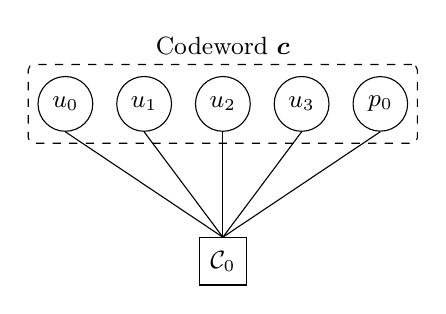
\begin{tikzpicture}%[scale=\tikzscale]
  \node[draw=black, circle, minimum height=0.6cm, text=black] (v1) at (0.0, 2.0) {\small{$u_0$}};
  \node[draw=black, circle, minimum height=0.6cm, text=black] (v2) at (1.0, 2.0) {\small{$u_1$}};
  \node[draw=black, circle, minimum height=0.6cm, text=black] (v3) at (2.0, 2.0) {\small{$u_2$}};
  \node[draw=black, circle, minimum height=0.6cm, text=black] (v4) at (3.0, 2.0) {\small{$u_3$}};
  \node[draw=black, circle, minimum height=0.6cm, text=black] (v5) at (4.0, 2.0) {\small{$p_0$}};

  \node[draw=black, rounded corners=2pt, minimum height=1cm, label={[black]above:\small{Codeword $\bm{c}$}}, dashed, fit=(v1) (v2) (v3) (v4) (v5)] (vn) {};

  \node[draw=black, minimum width=0.6cm, minimum height=0.6cm, text=black] (ca) at (2.0, 0.0) {\small{$\mathcal{C}_0$}};

  \draw (v1.south) -- (ca.north) node [midway, text=black] {};
  \draw (v2.south) -- (ca.north) node [midway, text=black] {};
  \draw (v3.south) -- (ca.north) node [midway, text=black] {};
  \draw (v4.south) -- (ca.north) node [midway, text=black] {};
  \draw (v5.south) -- (ca.north) node [midway, text=black] {};
  \end{tikzpicture}
\end{document}